% Options for packages loaded elsewhere
\PassOptionsToPackage{unicode}{hyperref}
\PassOptionsToPackage{hyphens}{url}
%
\documentclass[
]{article}
\usepackage{lmodern}
\usepackage{amssymb,amsmath}
\usepackage{ifxetex,ifluatex}
\ifnum 0\ifxetex 1\fi\ifluatex 1\fi=0 % if pdftex
  \usepackage[T1]{fontenc}
  \usepackage[utf8]{inputenc}
  \usepackage{textcomp} % provide euro and other symbols
\else % if luatex or xetex
  \usepackage{unicode-math}
  \defaultfontfeatures{Scale=MatchLowercase}
  \defaultfontfeatures[\rmfamily]{Ligatures=TeX,Scale=1}
\fi
% Use upquote if available, for straight quotes in verbatim environments
\IfFileExists{upquote.sty}{\usepackage{upquote}}{}
\IfFileExists{microtype.sty}{% use microtype if available
  \usepackage[]{microtype}
  \UseMicrotypeSet[protrusion]{basicmath} % disable protrusion for tt fonts
}{}
\makeatletter
\@ifundefined{KOMAClassName}{% if non-KOMA class
  \IfFileExists{parskip.sty}{%
    \usepackage{parskip}
  }{% else
    \setlength{\parindent}{0pt}
    \setlength{\parskip}{6pt plus 2pt minus 1pt}}
}{% if KOMA class
  \KOMAoptions{parskip=half}}
\makeatother
\usepackage{xcolor}
\IfFileExists{xurl.sty}{\usepackage{xurl}}{} % add URL line breaks if available
\IfFileExists{bookmark.sty}{\usepackage{bookmark}}{\usepackage{hyperref}}
\hypersetup{
  pdftitle={Chapter 4. Data Plots Peter smith},
  hidelinks,
  pdfcreator={LaTeX via pandoc}}
\urlstyle{same} % disable monospaced font for URLs
\usepackage[margin=1in]{geometry}
\usepackage{color}
\usepackage{fancyvrb}
\newcommand{\VerbBar}{|}
\newcommand{\VERB}{\Verb[commandchars=\\\{\}]}
\DefineVerbatimEnvironment{Highlighting}{Verbatim}{commandchars=\\\{\}}
% Add ',fontsize=\small' for more characters per line
\usepackage{framed}
\definecolor{shadecolor}{RGB}{248,248,248}
\newenvironment{Shaded}{\begin{snugshade}}{\end{snugshade}}
\newcommand{\AlertTok}[1]{\textcolor[rgb]{0.94,0.16,0.16}{#1}}
\newcommand{\AnnotationTok}[1]{\textcolor[rgb]{0.56,0.35,0.01}{\textbf{\textit{#1}}}}
\newcommand{\AttributeTok}[1]{\textcolor[rgb]{0.77,0.63,0.00}{#1}}
\newcommand{\BaseNTok}[1]{\textcolor[rgb]{0.00,0.00,0.81}{#1}}
\newcommand{\BuiltInTok}[1]{#1}
\newcommand{\CharTok}[1]{\textcolor[rgb]{0.31,0.60,0.02}{#1}}
\newcommand{\CommentTok}[1]{\textcolor[rgb]{0.56,0.35,0.01}{\textit{#1}}}
\newcommand{\CommentVarTok}[1]{\textcolor[rgb]{0.56,0.35,0.01}{\textbf{\textit{#1}}}}
\newcommand{\ConstantTok}[1]{\textcolor[rgb]{0.00,0.00,0.00}{#1}}
\newcommand{\ControlFlowTok}[1]{\textcolor[rgb]{0.13,0.29,0.53}{\textbf{#1}}}
\newcommand{\DataTypeTok}[1]{\textcolor[rgb]{0.13,0.29,0.53}{#1}}
\newcommand{\DecValTok}[1]{\textcolor[rgb]{0.00,0.00,0.81}{#1}}
\newcommand{\DocumentationTok}[1]{\textcolor[rgb]{0.56,0.35,0.01}{\textbf{\textit{#1}}}}
\newcommand{\ErrorTok}[1]{\textcolor[rgb]{0.64,0.00,0.00}{\textbf{#1}}}
\newcommand{\ExtensionTok}[1]{#1}
\newcommand{\FloatTok}[1]{\textcolor[rgb]{0.00,0.00,0.81}{#1}}
\newcommand{\FunctionTok}[1]{\textcolor[rgb]{0.00,0.00,0.00}{#1}}
\newcommand{\ImportTok}[1]{#1}
\newcommand{\InformationTok}[1]{\textcolor[rgb]{0.56,0.35,0.01}{\textbf{\textit{#1}}}}
\newcommand{\KeywordTok}[1]{\textcolor[rgb]{0.13,0.29,0.53}{\textbf{#1}}}
\newcommand{\NormalTok}[1]{#1}
\newcommand{\OperatorTok}[1]{\textcolor[rgb]{0.81,0.36,0.00}{\textbf{#1}}}
\newcommand{\OtherTok}[1]{\textcolor[rgb]{0.56,0.35,0.01}{#1}}
\newcommand{\PreprocessorTok}[1]{\textcolor[rgb]{0.56,0.35,0.01}{\textit{#1}}}
\newcommand{\RegionMarkerTok}[1]{#1}
\newcommand{\SpecialCharTok}[1]{\textcolor[rgb]{0.00,0.00,0.00}{#1}}
\newcommand{\SpecialStringTok}[1]{\textcolor[rgb]{0.31,0.60,0.02}{#1}}
\newcommand{\StringTok}[1]{\textcolor[rgb]{0.31,0.60,0.02}{#1}}
\newcommand{\VariableTok}[1]{\textcolor[rgb]{0.00,0.00,0.00}{#1}}
\newcommand{\VerbatimStringTok}[1]{\textcolor[rgb]{0.31,0.60,0.02}{#1}}
\newcommand{\WarningTok}[1]{\textcolor[rgb]{0.56,0.35,0.01}{\textbf{\textit{#1}}}}
\usepackage{graphicx,grffile}
\makeatletter
\def\maxwidth{\ifdim\Gin@nat@width>\linewidth\linewidth\else\Gin@nat@width\fi}
\def\maxheight{\ifdim\Gin@nat@height>\textheight\textheight\else\Gin@nat@height\fi}
\makeatother
% Scale images if necessary, so that they will not overflow the page
% margins by default, and it is still possible to overwrite the defaults
% using explicit options in \includegraphics[width, height, ...]{}
\setkeys{Gin}{width=\maxwidth,height=\maxheight,keepaspectratio}
% Set default figure placement to htbp
\makeatletter
\def\fps@figure{htbp}
\makeatother
\setlength{\emergencystretch}{3em} % prevent overfull lines
\providecommand{\tightlist}{%
  \setlength{\itemsep}{0pt}\setlength{\parskip}{0pt}}
\setcounter{secnumdepth}{-\maxdimen} % remove section numbering

\title{Chapter 4. Data Plots Peter smith}
\author{}
\date{\vspace{-2.5em}}

\begin{document}
\maketitle

\hypertarget{required-libraries}{%
\subsubsection{Required libraries}\label{required-libraries}}

\begin{Shaded}
\begin{Highlighting}[]
\KeywordTok{library}\NormalTok{(matlib)}
\end{Highlighting}
\end{Shaded}

\begin{verbatim}
## Warning: package 'matlib' was built under R version 4.0.4
\end{verbatim}

\begin{Shaded}
\begin{Highlighting}[]
\NormalTok{knitr}\OperatorTok{::}\KeywordTok{include_graphics}\NormalTok{(}\StringTok{"4_1.PNG"}\NormalTok{)}
\end{Highlighting}
\end{Shaded}

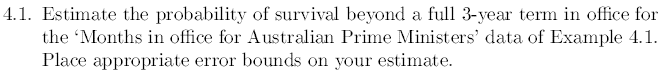
\includegraphics[width=9.19in]{4_1}

\hypertarget{required-data}{%
\subsubsection{Required data}\label{required-data}}

To facilitate the calculations, we will plot the empirical survival
function, first creating the vectors that store the data.

\begin{Shaded}
\begin{Highlighting}[]
\CommentTok{## Months in office for Australian Prime Ministers}

\NormalTok{ministers <-}\StringTok{ }\KeywordTok{c}\NormalTok{(}\KeywordTok{seq}\NormalTok{(}\DecValTok{1}\OperatorTok{:}\DecValTok{29}\NormalTok{))}
\NormalTok{months <-}\StringTok{ }\KeywordTok{c}\NormalTok{(}\DecValTok{33}\NormalTok{,}\DecValTok{8}\NormalTok{,}\DecValTok{5}\NormalTok{,}\DecValTok{12}\NormalTok{,}\DecValTok{41}\NormalTok{,}\DecValTok{8}\NormalTok{,}\DecValTok{11}\NormalTok{,}\DecValTok{39}\NormalTok{,}\DecValTok{16}\NormalTok{,}\DecValTok{14}\NormalTok{,}\DecValTok{89}\NormalTok{,}\DecValTok{81}\NormalTok{,}\DecValTok{28}\NormalTok{,}\DecValTok{88}\NormalTok{,}\DecValTok{1}\NormalTok{,}\DecValTok{29}\NormalTok{,}\DecValTok{3}\NormalTok{,}\DecValTok{46}\NormalTok{,}\DecValTok{1}\NormalTok{,}\DecValTok{54}\NormalTok{,}\DecValTok{194}\NormalTok{,}\DecValTok{24}\NormalTok{,}\DecValTok{2}\NormalTok{,}\DecValTok{39}\NormalTok{,}\DecValTok{22}\NormalTok{,}\DecValTok{36}\NormalTok{,}\DecValTok{89}\NormalTok{,}\DecValTok{106}\NormalTok{,}\DecValTok{52}\NormalTok{)}
\end{Highlighting}
\end{Shaded}

\hypertarget{plotting-position-calculations}{%
\subsubsection{Plotting position
calculations}\label{plotting-position-calculations}}

\begin{Shaded}
\begin{Highlighting}[]
\CommentTok{## Plotting position}

\NormalTok{p <-}\StringTok{ }\NormalTok{(ministers }\OperatorTok{-}\StringTok{ }\FloatTok{0.5}\NormalTok{)}\OperatorTok{/}\KeywordTok{length}\NormalTok{(ministers)}
\KeywordTok{head}\NormalTok{(p)}
\end{Highlighting}
\end{Shaded}

\begin{verbatim}
## [1] 0.01724138 0.05172414 0.08620690 0.12068966 0.15517241 0.18965517
\end{verbatim}

\hypertarget{data-plot}{%
\subsubsection{Data Plot}\label{data-plot}}

\begin{Shaded}
\begin{Highlighting}[]
\CommentTok{## Empirical survivor plot}

\NormalTok{months <-}\StringTok{ }\KeywordTok{sort}\NormalTok{(months)}
\NormalTok{data <-}\StringTok{ }\KeywordTok{as.data.frame}\NormalTok{(}\KeywordTok{cbind}\NormalTok{(months,}\DecValTok{1}\OperatorTok{-}\NormalTok{p))}
\KeywordTok{plot}\NormalTok{(months,}\DecValTok{1}\OperatorTok{-}\NormalTok{p, }\DataTypeTok{main=}\StringTok{"Empirical Survival Function"}\NormalTok{, }\DataTypeTok{xlab =} \StringTok{"Months in office"}\NormalTok{, }\DataTypeTok{ylab =} \StringTok{"Survival Probability"}\NormalTok{, }\DataTypeTok{col =}\StringTok{"red"}\NormalTok{)}
\end{Highlighting}
\end{Shaded}

\includegraphics{Cap_4_exercices_files/figure-latex/unnamed-chunk-5-1.pdf}

\hypertarget{estimate-probablity-of-survival-beyond-full-3-years}{%
\subsubsection{Estimate probablity of survival beyond full 3
years}\label{estimate-probablity-of-survival-beyond-full-3-years}}

Knowing that the estimate probability of the survival fucntion is giving
by:

\[S_n\left(y\right)=\frac{number\:of\:observations\:>y}{n}=\frac{1}{n}\sum _{i=1}^n\:I\left(y,\infty \right)\left(Y_i\right)\]

then:

\[S_{29}\left(36\right)=\frac{1}{29}\sum _{i=1}^n\:I\left(36,\infty \right)\left(Y_i\right)=\frac{12}{29}\:=\:0.4137\]
\#\#\# Confidence interval

And the approximate confidence interval based in two standard error is:

\[S_{29}\left(17\right)\frac{+}{ }2\sqrt{\frac{S_{29}\left(17\right)\left(1-S_{29}\left(17\right)\right)}{29}}\]

then

\[0.4137+2\sqrt{\frac{0.4137\left(1-0.4137\right)}{29}}=0.5966\]

and

\[0.4137-2\sqrt{\frac{0.4137\left(1-0.4137\right)}{29}}=0.2308\]

\begin{Shaded}
\begin{Highlighting}[]
\NormalTok{knitr}\OperatorTok{::}\KeywordTok{include_graphics}\NormalTok{(}\StringTok{"4_2.PNG"}\NormalTok{)}
\end{Highlighting}
\end{Shaded}

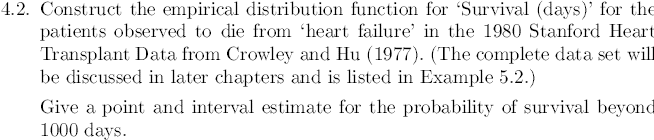
\includegraphics[width=9.08in]{4_2}

\hypertarget{required-data-1}{%
\subsubsection{Required data}\label{required-data-1}}

\begin{Shaded}
\begin{Highlighting}[]
\CommentTok{## Stanford Heart Transplat Data}

\CommentTok{## Reading data}
\NormalTok{heart <-}\StringTok{ }\KeywordTok{read.csv}\NormalTok{(}\StringTok{"heart_data.csv"}\NormalTok{, }\DataTypeTok{header=}\NormalTok{T,}\DataTypeTok{sep=}\StringTok{";"}\NormalTok{)}
\KeywordTok{attach}\NormalTok{(heart)}
\KeywordTok{head}\NormalTok{(heart)}
\end{Highlighting}
\end{Shaded}

\begin{verbatim}
##   Days Cens  Age   T5
## 1   15    1 54.3 1.11
## 2    3    1 40.4 1.66
## 3  624    1 51.0 1.32
## 4   46    1 42.5 0.61
## 5  127    1 48.0 0.36
## 6   64    1 54.6 1.89
\end{verbatim}

\hypertarget{plotting-position-calculations-1}{%
\subsubsection{Plotting position
calculations}\label{plotting-position-calculations-1}}

\begin{Shaded}
\begin{Highlighting}[]
\CommentTok{## Plotting position}

\NormalTok{patients <-}\StringTok{ }\KeywordTok{seq}\NormalTok{(}\DecValTok{1}\OperatorTok{:}\KeywordTok{length}\NormalTok{(Days))}
\NormalTok{p <-}\StringTok{ }\NormalTok{(patients }\OperatorTok{-}\StringTok{ }\FloatTok{0.5}\NormalTok{)}\OperatorTok{/}\KeywordTok{length}\NormalTok{(patients)}
\KeywordTok{head}\NormalTok{(p)}
\end{Highlighting}
\end{Shaded}

\begin{verbatim}
## [1] 0.007246377 0.021739130 0.036231884 0.050724638 0.065217391 0.079710145
\end{verbatim}

\hypertarget{data-plot-1}{%
\subsubsection{Data Plot}\label{data-plot-1}}

\begin{Shaded}
\begin{Highlighting}[]
\CommentTok{## Empirical survivor plot}

\NormalTok{i <-}\StringTok{ }\KeywordTok{order}\NormalTok{(heart}\OperatorTok{$}\NormalTok{Days)}
\NormalTok{heart <-}\StringTok{ }\NormalTok{heart[i,]}
\NormalTok{p <-}\StringTok{ }\DecValTok{1}\OperatorTok{-}\NormalTok{p}

\NormalTok{Days <-}\StringTok{ }\NormalTok{heart}\OperatorTok{$}\NormalTok{Days}
\NormalTok{Cens <-}\StringTok{ }\NormalTok{heart}\OperatorTok{$}\NormalTok{Cens}

\NormalTok{newHeart <-}\StringTok{ }\KeywordTok{as.data.frame}\NormalTok{(}\KeywordTok{cbind}\NormalTok{(Days,Cens,p))}
\NormalTok{newHeart <-}\StringTok{ }\KeywordTok{subset}\NormalTok{(newHeart, Cens}\OperatorTok{==}\DecValTok{1}\NormalTok{)}
\KeywordTok{plot}\NormalTok{(newHeart}\OperatorTok{$}\NormalTok{Days,newHeart}\OperatorTok{$}\NormalTok{p, }\DataTypeTok{main=}\StringTok{"Empirical S(t) Heart transplant"}\NormalTok{, }\DataTypeTok{xlab =} \StringTok{"}
\StringTok{Days since heart transplant"}\NormalTok{, }\DataTypeTok{ylab =} \StringTok{"Survival Probability"}\NormalTok{, }\DataTypeTok{col=}\StringTok{"red"}\NormalTok{)}
\end{Highlighting}
\end{Shaded}

\includegraphics{Cap_4_exercices_files/figure-latex/unnamed-chunk-9-1.pdf}

\hypertarget{estimate-probablity-of-survival-beyond-1000-days}{%
\subsubsection{Estimate probablity of survival beyond 1000
days}\label{estimate-probablity-of-survival-beyond-1000-days}}

\begin{Shaded}
\begin{Highlighting}[]
\CommentTok{## Looking on the data greater than 1000}

\KeywordTok{sum}\NormalTok{(heart}\OperatorTok{$}\NormalTok{Days }\OperatorTok{>}\StringTok{ }\DecValTok{1000}\NormalTok{)}
\end{Highlighting}
\end{Shaded}

\begin{verbatim}
## [1] 8
\end{verbatim}

Then by the definition 1.3:

\[S_{69}\left(1000\right)=\frac{1}{69}\sum \:_{i=1}^{69}\:I\left(1000,\infty \:\right)\left(Y_i\right)=\frac{8}{69}=0.1159\]
\#\#\#\# Confidence interval

The approximate confidence interval based in two standard error is:

\[0.1159+2\sqrt{\frac{0.1159\left(1-0.1159\right)}{69}}=0.1929\] and

\[0.1159-2\sqrt{\frac{0.1159\left(1-0.1159\right)}{69}}=0.0388\]

\begin{Shaded}
\begin{Highlighting}[]
\NormalTok{knitr}\OperatorTok{::}\KeywordTok{include_graphics}\NormalTok{(}\StringTok{"4_3.PNG"}\NormalTok{)}
\end{Highlighting}
\end{Shaded}

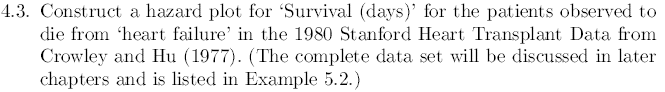
\includegraphics[width=9.24in]{4_3} \#\#\# Calculation of the empirical
and accumulative Hazard

\begin{Shaded}
\begin{Highlighting}[]
\NormalTok{k <-}\StringTok{ }\KeywordTok{seq}\NormalTok{(}\DecValTok{69}\NormalTok{,}\DecValTok{1}\NormalTok{)}
\NormalTok{Emp.h <-}\StringTok{ }\KeywordTok{c}\NormalTok{()}
\NormalTok{Days <-}\StringTok{ }\NormalTok{heart}\OperatorTok{$}\NormalTok{Days }
\NormalTok{Cens <-}\StringTok{ }\NormalTok{heart}\OperatorTok{$}\NormalTok{Cens}

\CommentTok{### The following cycles calculate all the data for the empirical risk, for ease of calculation the censored data are filled with zeros.}


\ControlFlowTok{for}\NormalTok{(i }\ControlFlowTok{in} \DecValTok{1}\OperatorTok{:}\DecValTok{69}\NormalTok{)\{}
  
  \ControlFlowTok{if}\NormalTok{(Cens[i] }\OperatorTok{==}\StringTok{ }\DecValTok{0}\NormalTok{)\{}
    
\NormalTok{    Emp.h[i]=}\StringTok{ }\DecValTok{0}

    
\NormalTok{  \}}\ControlFlowTok{else}\NormalTok{\{}
    
\NormalTok{    Emp.h[i] =}\StringTok{ }\DecValTok{1}\OperatorTok{/}\NormalTok{k[i]}

\NormalTok{  \}}
  
\NormalTok{\}}

\NormalTok{cum.H <-}\StringTok{ }\KeywordTok{cumsum}\NormalTok{(Emp.h)}

\ControlFlowTok{for}\NormalTok{(i }\ControlFlowTok{in} \DecValTok{1}\OperatorTok{:}\DecValTok{69}\NormalTok{)\{}
  
  \ControlFlowTok{if}\NormalTok{(Cens[i] }\OperatorTok{==}\StringTok{ }\DecValTok{0}\NormalTok{)\{}
    
\NormalTok{    cum.H[i]=}\StringTok{ }\DecValTok{0}

\NormalTok{  \}}
\NormalTok{\}}


\NormalTok{harzard.score<-}\StringTok{ }\KeywordTok{as.data.frame}\NormalTok{(}\KeywordTok{cbind}\NormalTok{(Days,Cens, k, Emp.h, cum.H))}

\KeywordTok{head}\NormalTok{(harzard.score)}
\end{Highlighting}
\end{Shaded}

\begin{verbatim}
##   Days Cens  k      Emp.h      cum.H
## 1    1    1 69 0.01449275 0.01449275
## 2    1    0 68 0.00000000 0.00000000
## 3    1    1 67 0.01492537 0.02941813
## 4    3    1 66 0.01515152 0.04456964
## 5   10    1 65 0.01538462 0.05995426
## 6   12    1 64 0.01562500 0.07557926
\end{verbatim}

\hypertarget{building-the-empirical-harzard-plot}{%
\subsubsection{Building the Empirical harzard
plot}\label{building-the-empirical-harzard-plot}}

\begin{Shaded}
\begin{Highlighting}[]
\CommentTok{### Building the graph}

\NormalTok{hz.plotting <-}\StringTok{ }\KeywordTok{subset}\NormalTok{(harzard.score, Cens }\OperatorTok{==}\StringTok{ }\DecValTok{1}\NormalTok{)}
\KeywordTok{plot}\NormalTok{(hz.plotting}\OperatorTok{$}\NormalTok{Days,hz.plotting}\OperatorTok{$}\NormalTok{Emp.h, }\DataTypeTok{main=}\StringTok{"Empirical Hazard Plot"}\NormalTok{, }\DataTypeTok{xlab =} \StringTok{"Days since heart transplant"}\NormalTok{, }\DataTypeTok{ylab =} \StringTok{"Hazard plot score"}\NormalTok{, }\DataTypeTok{col=}\StringTok{"red"}\NormalTok{)}
\end{Highlighting}
\end{Shaded}

\includegraphics{Cap_4_exercices_files/figure-latex/unnamed-chunk-13-1.pdf}

\begin{Shaded}
\begin{Highlighting}[]
\NormalTok{knitr}\OperatorTok{::}\KeywordTok{include_graphics}\NormalTok{(}\StringTok{"4_3_1.PNG"}\NormalTok{)}
\end{Highlighting}
\end{Shaded}

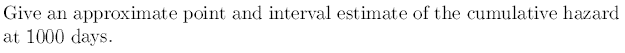
\includegraphics[width=8.68in]{4_3_1}

\begin{Shaded}
\begin{Highlighting}[]
\CommentTok{### Estimated accrued risk at 1,000 days, the closest point is 994 days.}

\NormalTok{hz.plotting}\OperatorTok{$}\NormalTok{cum.H[hz.plotting}\OperatorTok{$}\NormalTok{Days }\OperatorTok{==}\StringTok{ }\DecValTok{994}\NormalTok{]}
\end{Highlighting}
\end{Shaded}

\begin{verbatim}
## [1] 1.291767
\end{verbatim}

Based on the calculations in the table above, we can say that the
accumulated empirical hazard at 1000 days is 1.2918.

\begin{Shaded}
\begin{Highlighting}[]
\NormalTok{knitr}\OperatorTok{::}\KeywordTok{include_graphics}\NormalTok{(}\StringTok{"4_3_2.PNG"}\NormalTok{)}
\end{Highlighting}
\end{Shaded}

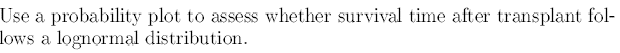
\includegraphics[width=8.61in]{4_3_2} \#\#\# Calculations of lognormal
probability distribution

\begin{Shaded}
\begin{Highlighting}[]
\NormalTok{inv_phi <-}\StringTok{ }\KeywordTok{qnorm}\NormalTok{(newHeart}\OperatorTok{$}\NormalTok{p)}
\NormalTok{result.lm <-}\StringTok{ }\KeywordTok{lm}\NormalTok{(inv_phi}\OperatorTok{~}\KeywordTok{log}\NormalTok{(newHeart}\OperatorTok{$}\NormalTok{Days))}

\KeywordTok{plot}\NormalTok{(}\KeywordTok{log}\NormalTok{(newHeart}\OperatorTok{$}\NormalTok{Days),inv_phi, }\DataTypeTok{main =} \StringTok{"Lognormal probability distribution for heart transplant"}\NormalTok{,}\DataTypeTok{xlab=}\StringTok{"log(Days)"}\NormalTok{, }\DataTypeTok{sub=}\StringTok{"log-normal"}\NormalTok{,}\DataTypeTok{ylab=}\KeywordTok{expression}\NormalTok{(Phi}\OperatorTok{^-}\DecValTok{1} \OperatorTok{*}\StringTok{ }\NormalTok{(}\KeywordTok{S}\NormalTok{(t))))}
\KeywordTok{abline}\NormalTok{(result.lm, }\DataTypeTok{col=}\StringTok{"red"}\NormalTok{)}
\end{Highlighting}
\end{Shaded}

\includegraphics{Cap_4_exercices_files/figure-latex/unnamed-chunk-17-1.pdf}

\begin{Shaded}
\begin{Highlighting}[]
\NormalTok{result.lm}
\end{Highlighting}
\end{Shaded}

\begin{verbatim}
## 
## Call:
## lm(formula = inv_phi ~ log(newHeart$Days))
## 
## Coefficients:
##        (Intercept)  log(newHeart$Days)  
##             2.4423             -0.4948
\end{verbatim}

Using the graph as empirical evidence, it can be corroborated that the
data are generated to fit a lognormal distribution( 2.4423 , -0.4948 ).

\hypertarget{accumulated-hazard-calculations}{%
\subsubsection{Accumulated hazard
calculations}\label{accumulated-hazard-calculations}}

Similarly, we can calculate the cumulative hazard for a log normal
distribution as follows:

\begin{Shaded}
\begin{Highlighting}[]
\NormalTok{Hexp <-}\StringTok{ }\DecValTok{1}\OperatorTok{-}\KeywordTok{exp}\NormalTok{(}\OperatorTok{-}\NormalTok{hz.plotting}\OperatorTok{$}\NormalTok{cum.H)}
\NormalTok{Hphi <-}\StringTok{ }\KeywordTok{qnorm}\NormalTok{(Hexp)}

\NormalTok{LogNomrh.lm <-}\StringTok{ }\KeywordTok{lm}\NormalTok{(Hphi}\OperatorTok{~}\KeywordTok{log}\NormalTok{(hz.plotting}\OperatorTok{$}\NormalTok{Days))}

\KeywordTok{plot}\NormalTok{(}\KeywordTok{log}\NormalTok{(hz.plotting}\OperatorTok{$}\NormalTok{Days),Hphi, }\DataTypeTok{main=}\StringTok{"Accumulated log−normal Hazard"}\NormalTok{, }\DataTypeTok{ylab =} \StringTok{"Accumulated log−normal Hazard"}\NormalTok{, }\DataTypeTok{xlab=}\StringTok{"log(Days)"}\NormalTok{, }\DataTypeTok{xlim=}\KeywordTok{c}\NormalTok{(}\DecValTok{0}\NormalTok{,}\DecValTok{7}\NormalTok{), }\DataTypeTok{ylim=}\KeywordTok{c}\NormalTok{(}\OperatorTok{-}\FloatTok{2.2}\NormalTok{,}\DecValTok{1}\NormalTok{) )}
\KeywordTok{abline}\NormalTok{(LogNomrh.lm, }\DataTypeTok{col=}\StringTok{"red"}\NormalTok{)}
\end{Highlighting}
\end{Shaded}

\includegraphics{Cap_4_exercices_files/figure-latex/unnamed-chunk-18-1.pdf}

\begin{Shaded}
\begin{Highlighting}[]
\NormalTok{knitr}\OperatorTok{::}\KeywordTok{include_graphics}\NormalTok{(}\StringTok{"4_4.PNG"}\NormalTok{)}
\end{Highlighting}
\end{Shaded}

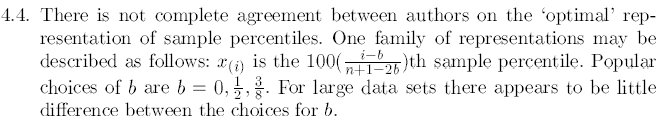
\includegraphics[width=9.22in]{4_4} In our case the author has decided
to use b = 0.5, as can be seen below:

\[100\left(\frac{i-b}{n+1-2b}\right)=100\left(\frac{i-\frac{1}{2}}{n+1-2\left(\frac{1}{2}\right)}\right)=100\left(\frac{i-\frac{1}{2}}{n}\right)\]

\end{document}
